\chapter{Introduction}
\section{Probability}



\begin{definition}{Independence}\vspace{-0.5cm}
	\begin{align*}
	X\perp Y \leftrightarrow p(X,Y)=p(X)p(Y)
	\end{align*}
\end{definition}
\begin{definition}{Conditional independence}\vspace{-0.5cm}
	\begin{align*}
	X\perp Y|Z \leftrightarrow p(X,Y|Z)=p(X|Z)p(Y|Z)
	\end{align*}
\end{definition}
All the dependencies between $X$ and $Y$ are mediated via $Z$. If $X$ and $Y$ are conditionally independent, then 
\begin{align*}
	p(X|Y,Z)&=\frac{p(X,Y|Z)}{p(Y|Z)}\\
	&=\frac{p(X|Z)p(Y|Z)}{p(Y|Z)}\\
	&=p(X|Z).
\end{align*}

\section{Gaussian Distribution}
For a $D$-dimensional vector $\rvx$, the multivariate Gaussian distribution takes the form
\begin{align*}
	\mathcal{N}(\mathbf{x}|\boldsymbol{\mu},\boldsymbol{\Sigma}) &= \frac{1}{(2\pi)^{D/2}|\boldsymbol{\Sigma}|^{1/2}}\exp\bigg(-\frac{1}{2}(\mathbf{x}-\boldsymbol{\mu})^T\boldsymbol{\Sigma}^{-1}(\mathbf{x}-\boldsymbol{\mu})\bigg)\\
\end{align*}


% \chapter{Bayesian}
\section{Naive Bayes}
\label{sec:naive_bayes}

  In this section, we discuss how to classify vectors of discrete-valued features $\mathbf{x}$. Recall that we discussed how to classify a feature vector $\mathbf{x}$ by applying Bayes rule to a generative classifier of the form 
  $$p(y=c|\mathbf{x},\boldsymbol{\theta})\propto p(\mathbf{x}|y=c, \boldsymbol{\theta})p(y=c|\boldsymbol{\theta})$$
  The key to using such models is specifying a suitable form for the class-conditional density $p(\mathbf{x}|y=c, \boldsymbol{\theta})$, which defines what kind of data we expect to see in each class. 
  \begin{itemize}
    \item  $\textbf{x} \in \{1,...,K\}^D$,
    \begin{itemize}
      \item $K$: the number of values for each feature.
      \item $D$: the number of features.
    \end{itemize}
    \item We will use a generative approach.
    \item Need to specify the class conditional distribution, $p(\mathbf{x}|y=c)$.
    \item A simple approach is to assume the features are \textbf{conditionally independence} given the class label.
		\begin{figure}[h]
			\centering
			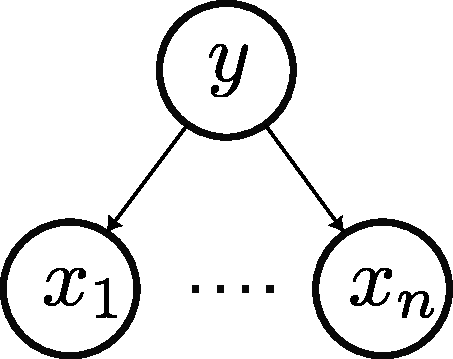
\includegraphics[scale=0.5]{./images/conditional_independence.pdf}
		\end{figure}
    \item This allows us to write the class conditional density as a product of one dimensional densities:
    $$p(\mathbf{x}|y=c, \boldsymbol{\theta}) = \prod_{j=1}^{D}p(x_j|y=c,\boldsymbol{\theta}_{jc})$$
  \end{itemize}
  The resulting model is called a \textbf{naive Bayes classifier (NBC)}. The model is called ``naive'' since we assume the independence between the features, which is not true in practice. However, if often results in classifiers that work well.

  The form of the class-conditional density depends on the type of each feature. We give some possibilities below:
  \begin{itemize}
    \item In the case of real-valued features, we can use the Gaussian distribution: $p(\mathbf{x}|y=c, \boldsymbol{\theta}) = \prod_{j=1}^{D}\mathcal{N}(x_j|\mu_{jc}^2)$, where $\mu_{jc}$ is the mean of feature $j$ in objects of class $c$, and $\sigma_{jc}^2$ is its variance.
    \item In the case of binary features, we can use the Bernoulli distribution: $p(\mathbf{x}|y=c, \boldsymbol{\theta}) = \prod_{j=1}^{D}\textrm{Ber}(x_j|\mu_{jc})$, where $\mu_{jc}$ is the probability that feature $j$ occurs in class $c$. This is sometimes called the \textbf{multivariate Bernoulli naive Bayes} model.
    \item In the case of categorical features, $x_j\in \{1,...,K\}$, we can model the multinomial distribution: $p(\mathbf{x}|y=c, \boldsymbol{\theta}) = \prod_{j=1}^{D}\textrm{Cat}(x_j|\mu_{jc})$, where $\boldsymbol{\mu}_{jc}$ is a histogram over the $K$ possible values for $x_j$ in class $c$.
  \end{itemize}

The probability for a single data case is given by
$$p(\mathbf{x}_i,y_i|\boldsymbol{\theta}) = p(y_i|\boldsymbol{\pi})\prod_{j}p(x_{ij}|\boldsymbol{\theta}_j)=\prod_{c}\pi_{c}^{\mathds{I}(y_i=c)}\prod_{j}\prod_{c}p(x_{ij}|\boldsymbol{\theta}_{jc})^{\mathds{I}(y_i=c)},$$
where $\boldsymbol{\pi}$ is a vector of class probability. Hence the log-likelihood is given by
	$$\textrm{log}p(\mathcal{D}|\boldsymbol{\theta}) = \sum_{c=1}^{C}N_c\textrm{log}\pi_c+\sum_{j=1}^{D}\sum_{c=1}^{C}\sum_{i:y_i=c}\textrm{log}p(x_{ij}|\boldsymbol{\theta}_{jc})$$

	\begin{algorithm}[H]
		\SetAlgoLined
%		\KwResult{Write here the result }
		Initialize $N_c=0,N_{jc}=0$ \;
		\For{$i=1:N$}{
      $c=y_i$ //Class label of $i$-th example;

      $N_c:=N_c+1$;

  		\For{$j=1:D$}{
      \uIf{$x_{ij}=1$}{
        $N_{jc}:=N_{jc}+1$
        }
  		}
		}
  $\hat{\pi}=\frac{N_c}{N},\hat{\theta}_{jc}=\frac{N_{jc}}{N_c}$
	\caption{Fitting a naive Bayes classifier to binary features}
\end{algorithm}

\section{Logistic Regression}
\label{sec:logistic_regression}

Logistic regression corresponds to the following binary classification model:
$$p(y|\mathbf{x},\mathbf{w})=\textrm{Ber}(y|\sigma(\mathbf{w}^T\mathbf{x}))$$

Logistic regression modles a logit (log odds) through a linear model. For binary data, the goal is to model the probability $p$ that one of two outcomes occurs. The logit function is $\textrm{log}\frac{p}{1-p}$, which varies between $-\infty$ and $+\infty$ as $p$ varies between $0$ and $1$.
$$\textrm{log}\frac{p}{1-p} = w_0x_0 +  w_1x_1 + ... + w_nx_n$$
Note that the logistic regression model assumes that the log-odds (\textit{logit}) of an observation $y$ can be expressed as a linear function. In this context, the logit function is called the \textbf{\textit{link function}} because it ``links'' the probability to the linear function of the predictor variables.

% Simplest solution to model a dependant variable $y$ is a linear regression. However, $y$ should be in a range of $[0,1]$. So we need to introduce the logit function. 

% The linear regression can be generalized to the classification setting with two changes:
% \begin{itemize}
% 	\item Replacing the Gaussian distribution for $y$ with a Bernoulli distribution: $p(y|\mathbf{x},\mathbf{w})=Ber(y|\mu(\mathbf{x}))$
% 	\item Squashing input data into sigmoid function $\sigma(\eta)$ that range from 0 to 1: $\sigma(\eta)\triangleq \frac{1}{1+exp(-\eta)}$.
% \end{itemize}
% $$p(y|\mathbf{x},\mathbf{w})=Ber(y|\sigma(\mathbf{w}^T\mathbf{x})),\$$

The negative log-likelihood for logistic regression is given by
\begin{align*}
	\textrm{NLL}(\mathbf{w}) &= -\sum_{i=1}^{N}\textrm{log}[\mu_i^{\mathds{I}(y_i=1)}\times (1-\mu_i)^{\mathds{I}(y_i=0)}]\\
	&=-\sum_{i=1}^{N}[y_i\textrm{log}\mu_i + (1-y_i) \textrm{log}(1-\mu_i)], \textrm{ }\footnotemark
\end{align*}
where $\mu=\sigma(\mathbf{w}^T\mathbf{x})$. This is also called \textbf{cross-entropy} error function. 
\footnotetext{$\mathds{I}(y_i=1) = y_i$, because $y_i\in \{0, 1\}$ is a binary variable}

Another way to express \textrm{NLL} is as follows. Suppose $\hat{y}_i\in\{-1,+1\}$ instead of $y_i\in\{0,1\}$. We have $p(y=1)=\frac{1}{1+\mathrm{exp}(-\mathbf{w}^T\mathbf{x})}$ and $p(y=-1)=\frac{1}{1+\mathrm{exp}(+\mathbf{w}^T\mathbf{x})}$. Hence
\begin{align*}
	\textrm{NLL}(\mathbf{w}) &= -\frac{1}{N}\sum_{n=1}^N [\mathbb{I}(\hat{y}_n=1)\log(\sigma(a_n))+\mathbb{I}(\hat{y}_n=-1)\log(\sigma(-a_n))]\\
							 &= -\frac{1}{N}\sum_{n=1}^N \log(\sigma(\hat{y}_na_n))\\
							 &=  \frac{1}{N}\sum_{i=1}^{N}\textrm{log}(1+\mathrm{exp}(-\hat{y}_i\mathbf{w}^T\mathbf{x}_i).
\end{align*}
Note that the sigmoid is used for compressing the output into $[0,1]$ and $\sigma(-a_n) = 1-\sigma(a_n)$. Unlike the linear regression, there is no closed from solution for logistic regression, thus we need optimization algorithms for it. Typically, optimization process involves the gradient and Hessian. 
\begin{align*}
	\mathbf{g}&=\frac{d}{d\mathbf{w}}\mathrm{NLL}(\mathbf{w})=\frac{d}{d\mu_i}\mathrm{NLL}(\mathbf{w})\frac{d\mu_i}{d\mathbf{h}}\frac{d\mathbf{h}}{d\mathbf{w}}\\
	& = \sum_{i=1}\Bigg[-\frac{y_i}{\mu_i} + \frac{(1-y_i) }{(1-\mu_i)}\Bigg]\frac{d\mu_i}{d\mathbf{h}}\frac{d\mathbf{h}}{d\mathbf{w}}=\sum_{i=1}\Bigg[\frac{\mu_i-y_i }{\mu_i(1-\mu_i)}\Bigg]\frac{d\mu_i}{d\mathbf{h}}\frac{d\mathbf{h}}{d\mathbf{w}}\\
	&=\sum_{i}(\mu_i-y_i)\mathbf{x}_i=\mathbf{X}^T(\boldsymbol{\mu}-\mathbf{y})\\
	\frac{d\mu_i}{d\mathbf{h}}& = \mu_i(1-\mu_i)\\
	\frac{d\mathbf{h}}{d\mathbf{w}}& = \mathbf{x}_i
\end{align*}
where $\mathbf{h}=\mathbf{w}^T\mathbf{x}$. 

We can also use the second-order method. 
\begin{align*}
\mathbf{H}&=\frac{d}{d\mathbf{w}}g(\mathbf{w})^T=\sum_{i}(\nabla_{\mathbf{w}}\mu_i)\mathbf{x}_i^T=\sum_{i}\mu_i(1-\mu_i)\mathbf{x}_i\mathbf{x}_i^T\\
&=\mathbf{X}^T\mathbf{S}\mathbf{X},
\end{align*}
where $\mathbf{S}\triangleq \mathrm{diag}(\mu_i(1-\mu_i))$. Note that $\mathbf{H}$ is positive definite, because the \textrm{NLL} is convex and has a global minimum. 



